%        File: survey.tex
%     Created: Thu Mar 16 10:00 PM 2017 C
% Last Change: Thu Mar 16 10:00 PM 2017 C
%

\documentclass[a4paper, 11pt]{article}

\title{Power Diagrams and Additively Weighted Voronoi Diagrams }
\date{4/24/17}
\author{Trevor Steil}

\usepackage{amsmath}
\usepackage{amsthm}
\usepackage{amssymb}
\usepackage[backend=biber,style=numeric,citestyle=numeric,style=numeric]{biblatex}
\usepackage[margin=1in]{geometry}
\usepackage{esint}
\usepackage{enumitem}
\usepackage{algorithm}
\usepackage{algorithmicx}
\usepackage{algpseudocode}
\usepackage{bbm}
\usepackage{xcolor}
\usepackage{tikz}
\usepackage{float}
\usepackage{wrapfig}
\usepackage{subcaption}

\newtheorem{theorem}{Theorem}[section]
\newtheorem{corollary}{Corollary}[section]
\newtheorem{proposition}{Proposition}[section]
\newtheorem{lemma}{Lemma}[section]
\newtheorem*{claim}{Claim}
%\newtheorem*{problem}{Problem}
%\newtheorem*{lemma}{Lemma}
\newtheorem{definition}{Definition}[section]

\newcommand{\R}{\mathbb{R}}
\newcommand{\N}{\mathbb{N}}
\newcommand{\C}{\mathbb{C}}
\newcommand{\Z}{\mathbb{Z}}
\newcommand{\Q}{\mathbb{Q}}
\newcommand{\E}{\mathbb{E}}
\newcommand{\supp}[1]{\mathop{\mathrm{supp}}\left(#1\right)}
\newcommand{\lip}[1]{\mathop{\mathrm{Lip}}\left(#1\right)}
\newcommand{\curl}{\mathrm{curl}}
\newcommand{\la}{\left \langle}
\newcommand{\ra}{\right \rangle}
\renewcommand{\vec}[1]{\mathbf{#1}}
\renewcommand{\div}{\mathrm{div}}

\newenvironment{problem}{\textbf{Problem.}}

\newenvironment{solution}[1][]{\emph{Solution #1}}

\algnewcommand{\Or}{\textbf{ or }}
\algnewcommand{\And}{\textbf{ or }}

\addbibresource{project.bib}

\begin{document}
\maketitle

\section{Introduction}
Voronoi diagrams provide a partitioning of space into regions where each region is defined by a \textit{site}. For a given site, its corresponding
region is defined as containing all points closer to that site than any other site. Voronoi diagrams have been studied as mathematical objects and as
computational tools providing solutions to many applied problems. Many generalizations and variations of Voronoi diagrams have also been studied in
similar ways.

\subsection{Definitions}

The closest-neighbors Voronoi diagram for a set of $n$ sites $S \subset \R^2$ partitions the plane into regions, or Voronoi cells, where each cell is associated to a
site $p \in S$ and is defined by
\begin{equation*}
  Vor(p) = \{ q \in \R^2 \ | \ d(p,q) < d(p',q) \text{ for all } p' \neq p \in S \} .
\end{equation*}
where $d(p,q)$ is the Euclidean distance between $p$ and $q$.

There are several ways to generalize this concept to give other interesting partitions of the plane. Partitioning into regions defined by sharing the
same $k$ closest sites in $S$ gives rise to an order-$k$ Voronoi diagram \cite{aurenhammer_survey}. When $k=n-1$, this gives the furthest-neighbor
Voronoi diagram.

Many other variations of Voronoi diagrams can be constructed through the use of weighted distance functions. Let $w: S \to \R^+$ be a function that defines
the weight of sites in $S$. The multiplicatively weighted Voronoi diagram partitions the plane into cells defined by
\begin{equation*}
  Vor_{mul}(p) = \left\{ q \in \R^2 \ \big| \ \frac{d(p,q)}{w(p)} < \frac{d(p',q)}{w(p')} \text{ for all } p' \neq p \in S \right\}.
\end{equation*}
These diagrams tend to be more difficult to study and are qualitatively very different from standard Voronoi diagrams. For example,
the boundaries between regions in multiplicatively weighted Voronoi diagrams form circular arcs \cite{ash-bolker}, and multiplicatively weighted Voronoi
cells can be disconnected and may partition the plane into $\Theta(n^2)$ connected components \cite{aurenhammer_survey}.

The additively weighted Voronoi diagram partitions the plane into cells defined by
\begin{equation*}
  Vor_{add}(p) = \left\{ q \in \R^2 \ | \ d(p,q) - w(p) < d(p',q) - w(p') \text{ for all } p' \neq p \in S \right\}.
\end{equation*}

A geometric object defined similarly to weighted Voronoi diagrams is the power diagram, which partitions the plane into power cells defined by
\begin{equation*}
  Vor_{pow}(p) = \{ q \in \R^2 \ | \ d^2(p,q) - w(p) \leq d^2(p',q) - w(p') \text{ for all } p' \neq p \in S \}.
\end{equation*}
For consistency, we will use $Vor_{pow}$ to denote power cells even though they are not given the name of Voronoi diagrams.
The distance function used in power diagrams is called the \textit{power function} and is denoted
$pow(q,p)$ where $q \in \R^2$ and $p \in S$.

The definitions of additively weighted Voronoi diagrams and power diagrams given above required $w(p)$ to be positive. This requirement is not
necessary because the definition of these Voronoi cells remains the same if any constant is added to $w(p)$ for all $p$. Requiring weights to be at
least nonnegative will make some of the following geometric relations easier to visualize.

In the remaining sections, additively weighted Voronoi diagrams and power diagrams will be the main consideration. We will use the term weighted
Voronoi diagram to refer to additively weighted Voronoi diagrams. Also, the definitions given above naturally extend to higher dimensions. We will
consider diagrams in $\R^2$, but many ideas and results will hold in higher dimensions as well. Some of these extensions and the differences they
present will be highlighted.

\subsection{Notation}

As defined above, we will let $Vor(p), Vor_{mul}(p), Vor_{add}(p),$ and $Vor_{pow}(p)$ denote the various Voronoi cells associated to a (weighted) site $p
\in S$. Similarly, we will use $Vor(S), Vor_{mul}(S), Vor_{add}(S),$ and $Vor_{pow}(S)$ to denote the various Voronoi diagrams of $S$. For two
cells $R$ and $R'$ sharing a boundary in any of the diagrams above, we define $\partial_{R R'}$ to be that boundary. Most often, we will talk of cells
associated to sites, in which case we will use $\partial_{pq} = \partial_{Vor(p) Vor(q)}$ for brevity. We will use $P: \R^3 \to \R^3$ to be the
orthogonal projection onto the plane $\{ z = 0 \}$. When convenient, we may identify $\R^2$ with the plane $\{ z=0 \} \subseteq \R^3$.

\subsection{Basic Geometric Results}
\label{sec:basic_geom}

The definition of additively weighted Voronoi diagrams has a useful geometric interpretation. For a site $p \in S$, let $\mathcal{D}_p$ be the disc of radius $w(p)$ centered at $p$. Then we
can define
\begin{equation*}
  Vor_{add}(p) = \left\{ q \in \R^2 \ | \ \min_{\tilde{p} \in \mathcal{D}_p} d(\tilde{p}, q) < \min_{\tilde{p}' \in \mathcal{D}_{p'}} d(\tilde{p}', q) \text{
  for all } p' \neq p \in S \right\},
\end{equation*}
that is, we can measure distances as the minimum distance to any point in the disc centered at a given site \cite{rosenberger_additive}.

We can similarly interpret power diagrams in terms of circles. For $p \in S$, consider a circle $C(p)$ of radius $r(p) = \sqrt{w(p)}$ centered at $p$. Using the
Pythagorean theorem, we can see for any point $q \in \R^2$, $pow(q,p) = d^2(p,q) - r^2(p)$ gives the distance from $q$ to the circle centered at $p$
measured along a line tangent to $C(p)$.

Using the above formulations, we may speak of weighted Voronoi diagrams and power diagrams by thinking of $S$ as
containing a set of sites in $\R^2$ with associated weights, or we may refer to $S$ as a set of circles with with centers at $\{p_i\}$ and radii given by the appropriate weights.
Whether we think of $S$ as sites with weights or circles in the plane, we will use $Vor_{add}(S)$ and $Vor_{pow}(S)$ to denote the
associated diagrams, and similarly for $Vor_{add}(p)$ and $Vor_{pow}(p)$.

It is worth noting that $p \in S$ is not necessarily contained in $Vor_{add}(p)$ or $Vor_{pow}(p)$. If $w(p') - w(p) > d(p,p')$, then $p \in
Vor_{add}(p')$. This can also be interpreted as the associated circles being very small relative to nearby circles. A similar statement holds for power diagrams.
Despite this difference, the Voronoi cells of weighted Voronoi diagrams and power diagrams are still connected, and there are $O(n)$ vertices, edges,
and faces in the diagrams \cite{aurenhammer_power} \cite{rosenberger_additive}.

Unlike the straight-line boundaries of standard
Voronoi diagrams, boundaries between regions in additively weighted Voronoi diagrams are hyperbolic arcs or straight line segments
\cite{aurenhammer_additive}, as seen in Figure \ref{fig:wgt}. This can be seen by noticing $d(x,p) - w(p) = d(x,q) - w(q)$ if and only if $d(x,p) - d(x,q) = w(p) - w(q)$, that is
points on $\partial_{pq}$ have the difference of distances between $p$ and $q$ equal to a constant, which defines a hyperbola.

For power diagrams, boundaries are straight like in standard Voronoi diagrams, as seen in Figure \ref{fig:pow}. Let $p, q \in S$ be circles with radii $r(p), r(q)$ respectively. The set of $s = (x,y) \in \R^2$ where $pow(s,p) = pow(s,q)$
is given by the line
\begin{equation*}
  y = -\frac{q_x - p_x}{q_y - p_y} x + \frac{1}{2(q_y - p_y)} \left(q_x^2 + q_y^2 - p_x^2 - p_y^2 - r^2(q) + r^2(p) \right),
  \label{eq:pow_intersect}
\end{equation*}
where $p = (p_x, p_y)$ and $q = (q_x, q_y)$ \cite{aurenhammer_power}. From this, it is apparent that the boundary between power cells is a straight line or line segment perpendicular to the
line that is perpendicular to the straight line through $p$ and $q$.

\begin{figure}[h]
  \centering
  \begin{subfigure}[t]{0.45 \textwidth}
    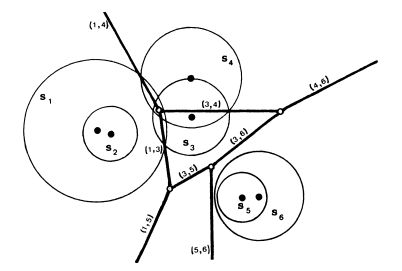
\includegraphics[height=2.25in]{power(aur_pow).png}
    \caption{Example power diagram (from \cite{aurenhammer_power})}
    \label{fig:pow}
  \end{subfigure}
  \begin{subfigure}[t]{0.47\textwidth}
    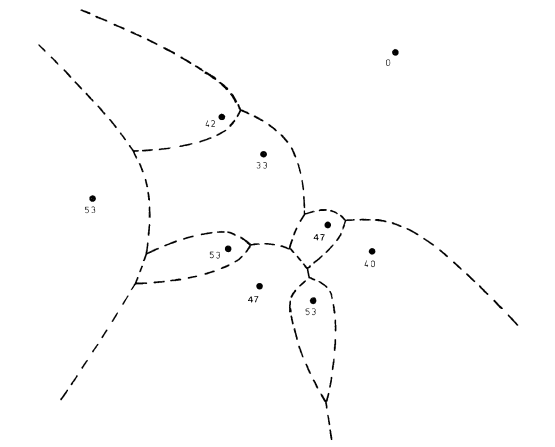
\includegraphics[height=2.25in]{weighted(aur_surv).png}
    \caption{Example weighted Voronoi diagram (from \cite{aurenhammer_survey})}
    \label{fig:wgt}
  \end{subfigure}
  \caption{}
\end{figure}

In the remainder of the paper, we will discuss connections between weighted Voronoi diagrams, power diagrams, and other geometric objects. After this,
we will use some of these connections to investigate the diagram recognition problem which starts with a partitioning of the plane and seeks to decide if the diagram could be the
weighted Voronoi diagram or power diagram for some set of sites and weights. Next, we will discuss algorithms for computing these diagrams, often with
explicit use of or motivation from the geometric connections we will establish. Following this, we will present a small number of applications of
weighted Voronoi diagrams and power diagrams to various areas.

\section{Relationships to Other Geometric Structures}
\label{sec:geom_rel}
The various Voronoi diagrams defined above have many connections to other geometric structures. A generalization of Delaunay triangulations can be
defined as the dual of these diagrams, but we will not discuss these here. Instead, our focus will be on connections between weighted Voronoi
diagrams, power diagrams, and 3-dimensional objects.

\subsection{Cone Arrangements}
\label{sec:cone}
For motivation, we will first consider a standard Voronoi diagram. Take a site $p \in S$. Define
\[ C_p = \{ (x, y, d(p, (x,y)) \}. \]
This defines a cone with vertex at $p$ in the $xy$-plane. Looking at the cones for all sites in $S$, we can see that $Vor(p)$ is the region in $\R^2$ corresponding to the height of $C_p$ being
less than the height of all other cones. If we look at the intersection of two cones for $p \neq q$, we have
\[ C_p \cap C_{q} = \{ (x,y,z) | z = d(p, (x,y)) = d(q, (x,y)) \}. \]
Projecting orthogonally onto the plane $\{z = 0\}$, $P(C_p \cap C_{q})$ gives the points in the plane that are equidistant to $p$ and $q$. This projection therefore contains
$\partial_{pq}$ in the Voronoi diagram.

A segment of $P( C_p \cap C_q)$ is not in $\partial_{pq}$ if and only if the projected segment is contained in the interior of $Vor(p')$ for $p'
\neq p, q$. This corresponds to $C_{p'}$ lying below $C_p \cap C_q$.

We can apply the same reasoning to weighted Voronoi diagrams, where we define
\[ C_p = \{ (x, y, d(p, (x,y)) - w(p) \}. \]
This now gives cones that are shifted vertically by $w(p)$ units.  When $w(p) \geq 0$ for some $p \in S$, we see $C_p \cap \{ z = 0 \}$ is the circle
centered at $p$ described in Section \ref{sec:basic_geom}.

Now $Vor_{add}(p)$ is given by $P(C_p)$ on the region where $C_p$ is below all other
cones. We also get a similar description of $\partial_{pq}$ as in the standard Voronoi case.

These cones can also used to describe regions in order-$k$ weighted Voronoi diagrams by not looking at intersections of cones where no other
cone lies below the intersection, but by looking for intersections where $k-1$ other cones lie below the intersection \cite{rosenberger_additive}.

The visualization as cones allows us to easily see that it is not necessarily the case that $p \in Vor_{add}(p)$. If we shift a cone up far enough, it
will lie completely inside another cone, giving $p \notin Vor_{add}(p)$. This is equivalent to the previous description that $p \notin Vor_{add}(p)$
if $w(p') - w(p) > d(p,p')$ for some $p' \in S$.

\subsection{Weighted Voronoi Diagrams and Power Diagrams}

Weighted Voronoi diagrams can be relateed to power diagrams through an embedding of weighted Voronoi diagrams in $\R^2$ into power diagrams in $\R^3$.
This embedding process applies more generally and requires a few definitions.

To begin with, we will state the result for general distance functions. Take $S \subset \R^2$ to be our sites. Any function $f: \R^2 \times S \to \R$
can be considered as a distance function that allows us to measure the distance between points in the plane and any of the sites. Using this distance
function, we can construct a Voronoi diagram, $Vor(S,f)$.

Let $F: \R \to \R$ be a strictly increasing function. For $p,q \in S \subset \R^2$, we define
\[ cone_F(p) = \{ (x,y,z) | (x,y) \in \R^2, z = F( f( (x,y), p) ) \}. \]

We call a diagram \textit{affinely transformable} if there is a function $F$ as above such that $cone_F(p) \cap cone_F(q)$ is contained in a plane in $\R^3$ for any distinct
$p,q \in S$.

Let $V$ be a Voronoi diagram in $\R^3$. We say the 2-dimensional Voronoi diagram $V(S,f)$ can be \textit{embedded} in $V$ if for some $F$ as above,
there is a cell $C$ of $V$ for each $p \in S$ such that $P( C \cap cone_F(p)) = Vor(p)$, where $P$ is the orthogonal projection onto the plane $\{ z =
0 \}$ and we have used $Vor(p)$ to mean the region defined
by the distance function $f$, not necessarily a region defined for a standard Voronoi diagram.

We have the following relation between affinely transformable diagrams and power diagrams:

\begin{theorem}
  \label{thm:affine}
  A Voronoi diagram $V(S,f)$ in $\R^2$ is affinely transformable if and only if it can be embedded into a power diagram in $\R^3$
  \cite{aurenhammer_additive}.
\end{theorem}

As an example, all weighted Voronoi diagrams in $\R^2$ can be embedded in power diagrams in $\R^3$. We take $f(q,p) = d(q,p) - w(p)$ to be the
distance function defining weighted Voronoi diagrams, and $F(x) = x$. In this case, $cone_F(p)$ is the cone described in Section \ref{sec:cone} for $p \in
S$. As already noted, the boundaries between cells in weighted Voronoi diagrams are hyperbolic arcs. The intersections $cone_F(p) \cap cone_F(q)$
are these arcs lifted back up to
the cones, which will each be contained in a single plane in $\R^3$.

By definition, we have that weighted Voronoi diagrams are affinely transformable by the above reasoning. By Theorem \ref{thm:affine}, weighted Voronoi
diagrams can be embedded in power diagrams in $\R^3$. In fact, the corresponding power diagram is given by sites $T = \{ (p, w(p)) | p \in S \}$ and
weights $\omega(p) = 2 w(p)^2$, where $S \subset \R^2$ and $w(p)$ are the sites and weights for the weighted Voronoi diagram
\cite{aurenhammer_additive}. This embedding result states that for any weighted Voronoi diagram, there is a power diagram in $\R^3$ such that
intersections of faces of the power diagram with the cones from Section \ref{sec:cone} can be projected into the plane $\{ z = 0 \}$ to give the faces
cells of the weighted Voronoi diagram.

\subsection{Convex Hulls}
\label{sec:conv}

There is an equivalence between power diagrams in $\R^2$ and lower convex hulls in $\R^3$. We will first show the correspondence between power diagrams and
upper envelopes and then use a correspondence between upper envelopes and lower convex hulls. To show this, we will modify the argument in
\cite{comp_geom} to hold for power diagrams rather than standard Voronoi diagrams by using tools from \cite{aurenhammer_power}. As we will see later, this correspondence can be useful
for algorithmically finding power diagrams.

First, we will need a few definitions. Let $U$ be the unit paraboloid in $\R^3$ defined as $U := (z = x^2 + y^2)$ for $(x,y) \in \R^2$.

Let $H$ be a finite set of nonvertical planes in $\R^3$. Considering the height of a plane as a function of coordinates in the $xy$-plane, we denote points
on the plane $h \in H$ as $(x,y,h(x,y))$. We define the \textit{upper envelope} of $H$ to be the object obtained by taking the plane with highest
$z$-coordinate above every point in the plane $\{ z = 0 \}$, that is,
\[ \mathcal{UE}(H) = \{ (x,y,z) | (x,y) \in \R^2, \ z = \max_{h \in H} h(x,y) \} .\]

Consider a set of sites $S \subset \R^2$ with associated radii $\{r(p) \ | \ p \in S\}$. For $p \in S$, we define $\Pi(p)$ to be the plane given by
\[ \Pi(p) : z = 2 p \cdot x - p^2 + r^2(p) ,\]
where $p^2$ is used to denote $p \cdot p$. The action of $\Pi$ is illustrated in Figure \ref{fig:lift}. It can be shown that $\Pi$ is a bijection between spheres in $\R^2$ and nonvertical planes in $\R^3$ which
intersect $U$. Intuitively, if we consider a site with $r(p) = 0$, then $\Pi(p)$ is tangent to $U$, fixing the normal vector to $\Pi(p)$. For $f(x) =
x \cdot x$, $\nabla f(x) = 2x$, so a plane with any nonhorizontal normal vector can be found. Adding arbitrary constants shifts the obtained planes, to allow any
nonvertical plane. In the definition of $\Pi(p)$, $r^2(p)$ is being added, which must be a positive number. This limits the only translations of
tangent planes of $U$ to be such that an intersection with $U$ is maintained.

\begin{figure}[h]
  \centering
  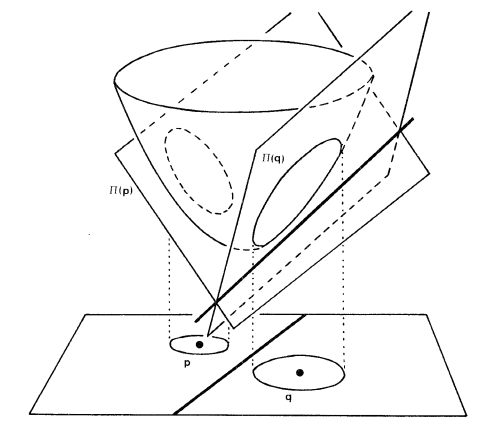
\includegraphics[height=3in]{lifting(aur_surv).png}
  \caption{The lifting map $\Pi$}
  \label{fig:lift}
\end{figure}

Now, we can begin to prove the correspondence between power diagrams and upper envelopes. First, we show the usefulness of the unit paraboloid $U$ in
relation to the power function.

\begin{lemma}
  \label{lem:proj}
  Let $q \in \R^2$ and $p \in S$. Let $q'$ be the vertical projection of $q$ onto $U$ and $q''$ be the vertical projection of $q$ onto $\Pi(p)$. Then
  $pow(q, p) = d(q, q') - d(q, q'')$.
\end{lemma}
\begin{proof}
  The projections to get $q'$ and $q''$ are both vertical projections, so we only need to find the heights of $q'$ and $q''$. By
  definition of $U$, the height of $q'$ is
  \[ q_z' = q^2.\]
  Also, by definition of $\Pi(p)$, the height of $q''$ is
  \[ q_z'' = 2p \cdot q - p^2 + r^2(p) . \]
  Therefore,
  \begin{align*}
    d(q,q') - d(q,q'') &= q'_z - q''_z \\
    &= q^2 - 2 p \cdot q + p^2 - r^2(p) \\
    &= (p-q)^2 - r^2(p) \\
    &= pow(q,p)
  \end{align*}
\end{proof}

Now we are able to prove the correspondence.

\begin{theorem}
  Let $H = \{ \Pi(p) \ | \ p \in S \}$. Then the projection of $\mathcal{UE}(H)$ on the plane $\{ z=0 \}$ is the power diagram of $S$.
  \label{thm:ue_to_pow}
\end{theorem}
\begin{proof}
  We must show $Vor_{pow}(p)$ is exactly the projection of the facet $\mathcal{UE}(H)$ that is part of $\Pi(p)$.

  Take $q \in Vor_{pow}(p)$. Then by assumption, $pow(q,p) \leq pow(q,\tilde{p})$ for all $\tilde{p} \in S$. To use Lemma \ref{lem:proj}, we let $q_p''$ be the
  vertical projection of $q$ onto $\Pi(p)$, and $q_{\tilde{p}}''$ be the vertical projection of $q$ onto $\Pi(\tilde{p})$. We notice the vertical projection
  of $q$ onto $U$ is independent of $p$ and $\tilde{p}$, so we leave this as $q'$. By Lemma \ref{lem:proj},
  \begin{align*}
    d(q,q') - d(q,q_p'') &= pow(q,p) \\
    &\leq pow(q,\tilde{p}) \\
    &= d(q,q') - d(q,q_{\tilde{p}}'')
  \end{align*}
  Therefore, $d(q,q_p'') \geq d(q, q_{\tilde{p}}'')$. Because the projections are vertical, $d(q,q_p'')$ and $d(q, q_{\tilde{p}}'')$ are the heights of
  $\Pi(p)$ and $\Pi(\tilde{p})$ above $q$. Thus, the height of $\Pi(p)$ is greater than or equal to the height of $\Pi(\tilde{p})$ above $q$ for all
  $\tilde{p} \in S$. This means $\Pi(p)$ is in $\mathcal{UE}(H)$ above $q$, as we needed to show.
\end{proof}

Let $H = \{ h_1,\dots, h_n \}$ be a set of planes in $\R^2$ that intersect $U$. Because $\Pi$ is a bijection, we can find a circle centered at $p_i$
with radius $r_i$ such that $\Pi( p_i ) = h_i$. Then $H = \{ \Pi(p_i) \}$, and by Theorem \ref{thm:ue_to_pow}, the projection of $\mathcal{UE}(H)$ gives the
power diagram of the set of circles $S = \{ p_i \}$. By Lemma \ref{lem:proj}, a point $(x,y,z) \in h_i$ is part of $\mathcal{UE}(H)$ if and only if $(x,y) \in
Vor_{pow}(p_i)$. Combining this with Theorem \ref{thm:ue_to_pow}, we know the cells of a power diagram can be encoded in an upper envelope and the
faces of an upper envelope can be given by a power diagram. We notice that in retrieving the faces of an upper envelope from a power diagram, the
power diagram on its own gives no information about the height of the upper envelope. This flexibility in being able to vertically shift upper
envelopes corresponds to a power diagram remaining unchanged when adding a constant to the radii of all circles.

The requirement that planes intersect $U$ can be removed, by vertically shifting the entire set of planes. Alternatively, by dropping the
interpretation of power diagrams being built on circles, we can consider power diagrams in which weights are allowed to be negative. This essentially
allows the $r^2$ to be negative in the definition of $\Pi$. This is summarized in the following.

\begin{corollary}
  There is a correspondence between power diagrams in $\R^2$ and upper envelopes of sets of nonvertical planes in $\R^3$ (up to a translation).
  \label{cor:ue_pow}
\end{corollary}

This result is a strengthening of results for standard Voronoi diagrams. For Voronoi diagrams, a set of planes can be found for which the projection
of the upper envelope gives rise to the Voronoi diagram, but the reverse direction is not always possible. This is due to the map $\Pi$ sending points
to planes that are tangent to $U$ when all weights are zero. In the case that a set of planes can be shifted so that all are tangent to $U$, a Voronoi diagram containing the
information of the upper envelope can be found. Otherwise, a power diagram is necessary.

This completes the correspondence between upper envelopes in $\R^3$ and power diagrams in $\R^2$. Now we must show the duality of lower convex hulls
and upper envelopes in $\R^3$. Let $h: z = ax + by + c$ be a plane in $\R^3$. As in \cite{aurenhammer_power}, we define
\begin{equation}
  \Delta(h) = \left( a, b, -c \right).
  \label{eq:duality1}
\end{equation}
This defines a map from nonvertical planes in $\R^3$ to points in $\R^3$. For a point $p \in \R^3$, we define
\begin{equation}
  \Delta(p) = \bigcup_{h \supseteq p} \Delta(h),
  \label{eq:duality2}
\end{equation}
where $h$ is ranging over all nonvertical planes containing $p$. This defines a map from points in $\R^3$ to planes in $\R^3$. For a point $p = (p_1, p_2, p_3)$,
by writing out the general form of a plane through $p$, this is equivalent to
\begin{equation}
  \Delta(p) := (z = p_1 x + p_2 y - p_3).
  \label{eq:duality3}
\end{equation}

We are able to use the same definition as above to map lines to lines, that is, for a line $l$ in $\R^3$, we define
\begin{equation}
  \Delta(l) = \bigcup_{h \supseteq l} \Delta(l).
  \label{eq:duality4}
\end{equation}

From the forms of \eqref{eq:duality1} and \eqref{eq:duality3}, it is clear that $\Delta$ is an involution. These operations can be thought of as
taking the plane $h: z = ax + bx - c$ and switching from $(a,b,c)$ as being coefficients and $(x,y,z)$ as being variables to $(x,y,z)$ being
coefficients and $(a,b,c)$ as being variables. From here, we can see these transformations are incidence and order preserving, that is, $p \in h$ if and only if
$\Delta(h) \in \Delta(p)$ and $p$ is above $h$ if and only if $\Delta(h)$ is above $\Delta(p)$. For these reasons, $\Delta$ gives a useful dual
correspndence between points and planes in $\R^3$.

Consider a set of points $T \subseteq \R^3$. $p \in T$ is on the lower convex hull of $T$ if and only if there is a plane $h$ with $p \in h$ and $h$
is below $p'$ for all $p' \in T$. Using the order-preserving property of the duality transformation, this occurs if and only if there is an $h$ with $\Delta(h) \in
\Delta(p)$ and $\Delta(p')$ is below $\Delta(h)$ for all $p' \in T$. This last statement characterizes $\Delta(p)$ being in the upper envelope of a set of
planes, giving the duality of lower convex hulls and upper envelopes in $\R^3$.

Combining the correspondence between power diagrams and upper envelopes given in Corollary \ref{cor:ue_pow} with this duality, we have the following:

\begin{theorem}
  Power diagrams in $\R^2$ correspond to lower convex hulls in $\R^3$.
  \label{thm:ch_pow}
\end{theorem}

All of the results above were stated for power diagrams in $\R^2$ and upper envelopes and convex hulls in $\R^3$. It is easy to see these results can
be extended to power diagrams in $\R^d$ and upper envelopes and convex hulls in $\R^{d+1}$ \cite{aurenhammer_power}.

\section{Diagram Recognition}

Up until this point, we have considered using a set of sites with associated weights to construct diagrams. We can instead take a diagram and decide
if it could have been constructed from a set of sites and weights. The general answer to this question is that given a diagram where it is already
known a set of possible sites exists, weights can be found for the sites which result in the given diagram \cite{ash-bolker}.

\subsection{Power Diagram Recognition}

For any power diagram, we have seen the boundary between two power cells is a straight line segment or ray that is perpendicular to the line between
the associated sites. In order to prove a partitioning of the plane arises as the power diagram of a set of sites and weights, we will require the
partition to have sites such that the above orthogonality holds.

Let $R = \{ R_1,\dots, R_n \}$ be a partition of the plane into convex regions with edges that are straight line segments and rays. Let $S = \{ p_1,
\dots, p_n \}$ be a set of points with $p_i$ corresponding to $R_i$ for all $i$. Let
\[ E = \{ (s_i, s_j) \ | \ R_i \text{ and } R_j \text{ are neighboring regions } \} . \]
The graph $G = (S,E)$ is a \textit{reciprocal figure} for $R$ if every edge $(s_i, s_j) \in E$ is perpendicular to $\partial_{R_i R_j}$,
and if you follow the ray from $s_i$ through $s_j$, you end up on the same side of the edge between $R_i$ and $R_j$ as $R_j$.

The last requirement is included to require cells to be convex, and edges intersecting at a vertex do so at an angle strictly less than $\pi$ radians.
The important requirement is pertaining to the orthogonality of line segments. It asserts the existence of a set of potential sites that satisfy the
orthogonality between edges and lines containing sites that all power diagrams exhibit. This can also be seen as requiring the existence of a dual
graph of $R$ satisfying the orthogonality constraint.

With the above definition, we get the following result.

\begin{theorem}
  A partition of the plane $R$ as above can be obtained as a power diagram of sites with weights if and only if $R$ has a reciprocal figure
  \cite{ash-bolker}.
  \label{thm:pow_rec}
\end{theorem}

As noted above, the existence of a reciprocal figure gives a set of sites to use for the power diagram. The theorem tells us we can find suitable
weights to use. This can be proved by looking locally at a vertex of $R$ and showing the weights can be solved for locally. By walking over the edges
of the reciprocal figure, we can successively find appropriate weights using the local result.

The local result we give requires vertices of the original partition to have degree exactly 3. This restriction can be lifted, but proof of this fact
will not be given (see \cite{ash-bolker}).

\begin{lemma}
  Let $R$ be a partition as above with three regions, $R_1, R_2$, and $R_3$, and a single vertex $v$. Let $p_1, p_2,$ and $p_3$ be vertices of a reciprocal figure of $R$. Then there exist weights
  $w_1, w_2, w_3$ such that $R$ is the power diagram associated to $S = \{ p_1, p_2, p_3 \}$.
  \label{lem:rec_loc}
\end{lemma}

\begin{proof}
  The proof presented here follows the proof of Lemma 10 in \cite{ash-bolker} but is adapted to using upper envelopes as discussed in Section
  \ref{sec:conv}.

  Initially, consider $w_1 = w_2 = w_3 = 0$. Then $\Pi(p_i)$ lifts $p_i$ to a plane tangent to the unit paraboloid $U$ as in Section \ref{sec:conv}.
  $P(\Pi(p_1) \cap \Pi(p_2))$ is a line that is the perpendicular bisector of $\overline{p_1 p_2}$ where $P$ is the vertical projection. Adding weights to $p_1$
  or $p_2$ maintains orthogonality while shifting the intersection of the $P(\Pi(p_1) \cap \Pi(p_2))$ with $\overline{p_1 p_2}$. This
  allows $w_1$ and $w_2$ to be found such that $P(\Pi(p_1) \cap \Pi(p_2)) \supseteq \partial_{R_1 R_2}$. It is worth noting the solution $(w_1, w_2)$
  is not unique.

  With $w_2$ now fixed, we can also find $w_3$ such that $P(\Pi(p_2) \cap \Pi(p_3)) \supseteq \partial_{R_2 R_3}$. Now $w_1, w_2,$
  and $w_3$ have been found. We must show $P(\Pi(p_1) \cap \Pi(p_3)) \supseteq \partial_{R_1 R_3}$.

  As before, $P(\Pi(p_1) \cap \Pi(p_3))$ is perpendicular to $\overline{p_1 p_3}$. Because $v \in \partial_{R_1 R_2} \cap \partial_{R_2
  R_3}$, $\tilde{v} \in \Pi(p_1) \cap \Pi(p_2) \cap \Pi(p_3)$ for some $\tilde{v}$ that projects onto $v$. Therefore, $\tilde{v} \in \Pi(p_1) \cap
  \Pi(p_3)$, and $v \in P(\Pi(p_1) \cap \Pi(p_3))$. Because $P(\Pi(p_1) \cap \Pi(p_3))$ is parallel to $\partial_{R_1 R_3}$ and they both contain $v$, $P(\Pi(p_1) \cap \Pi(p_3)) \supseteq \partial_{R_1 R_3}$.
\end{proof}

To prove Theorem \ref{thm:pow_rec}, we can take any initial vertex $p_i$ of the reciprocal figure. We can then walk along all edges of the reciprocal
figure and successively find appropriate weights as we reach new vertices for the first time. By Lemma \ref{lem:rec_loc}, solving in this way leads to
compatible weights at each step. After finishing, weights will be found for every site in the reciprocal figure $S$ such that the power diagram
associated to $S$ is $R$.

\subsection{Weighted Voronoi Diagram Recognition}

The boundaries between regions in weighted Voronoi diagrams are given by hyperbolic arcs. Hyperbolas are defined as being the set of points $x$ such
that $d(p,x) - d(q,x) = a$ for some constant $a$, where $p$ and $q$ are the foci of the hyperbola. In the case of weighted Voronoi diagrams, the foci
are the sites, and the constant $a$ is determined by the difference between the associated weights. This motivates the condition we desire for a
partition with boundaries given by hyperbolic arcs to be a weighted Voronoi diagram for some sites and weights.

\begin{theorem}
  \label{thm:add_rec}
  Let $R$ be a partition of $\R^2$ into regions separated by hyperbolic arcs where at least one arc is not a straight line. $R$ is the additively
  weighted Voronoi diagram for some points and weights if and only if the hyperbolic arcs bounding each region have a common focus in that region, and
  if any arcs are given by a straight line $L$, the foci corresponding to the regions bordering $L$ are equidistant from $L$ \cite{ash-bolker}.
\end{theorem}

As in power diagram recognition, this result states that if a set of potential sites exists, then weights can be found such that the weighted Voronoi
diagram corresponding to the sites and weights exactly coincides with the partition $R$. This result can be proved for more general partitions through
the use of cohomology.

\section{Algorithms}

\subsection{Fortune's Sweepline Algorithm}

We begin with a description of Fortune's algorithm for computing Voronoi diagrams. Following this, we will give interpretations of this algorithm in
terms of cone arrangements. From here we will describe the changes necessary to adapt Fortune's algorithm to computing an additively weighted Voronoi
diagram.

The obvious obstacle with developing a sweepline algorithm for computing Voronoi diagrams is that sites will be reached by a sweepline in the middle
of its Voronoi cell. Therefore, the algorithm must have some way of identifying the creation of a new cell before it has reached a site. One method of
doing this is to perform a transformation that maps a site to the bottom of its Voronoi cell. A sweepline algorithm could then identify new cells as
they are formed and compute a transformed Voronoi diagram. After this transformed Voronoi diagram has been completed, the Voronoi diagram can be
obtained by inverting the previous transformation considered \cite{fortune_sweepline}.

Another way of interpreting Fortune's algorithm is using a sweepline and a beach line. We will give an overview of this associated algorithm. Many
details and proofs will not be covered, but they can be found in \cite{comp_geom}.

\subsubsection{Algorithm Description}
The idea behind this approach is to use a
horizontal sweepline, $l$, that sweeps down the plane, while the beach line follows behind the sweepline and determines the boundary between the portion of the Voronoi diagram that cannot be
changed by anything past $l$ and the region that can still change.

To understand the structure of the beach line, we must understand what points in the plane will not be affected by any sites past $l$.
Consider a single site $p_i$ and point $q$ above $l$. If $d(p_i,q) < d(q,l)$, where $d(q,l)$ is understood to be the distance between $q$ and its
orthogonal projection onto $l$, then
no site not already reached by $l$ can be closer to $q$ than $p_i$ is. Similarly, if $d(p_i,q) > d(q,l)$, then a site just
below the sweepline could be closer to $q$ than $p_i$ is. The boundary between these two regions is the set of points that are equidistant from $p_i$ and
$l$. Therefore, this boundary is a parabola.

This gives a parabola for each site $p_i \in S$. Considering all sites at once, a point $q$ can only be changed by a site below $l$ if $d(p,q) > d(q,l)$ for all
currently known sites $p$. Therefore, the beach line is given by the bottom of the parabolas obtained for each individual site.

If we look at the intersection of two parabolic arcs on the beach line, these points will be equidistant from the sites associated to each parabolic
arc and $l$. This means as the sweep line moves, the beach line changes behind it and traces out the edges of the Voronoi diagram. To compute the
Voronoi diagram, we then need to understand how the beach line changes as new parabolic arcs form and old parabolic arcs disappear.

Parabolic arcs can only be added when $l$ reaches a new site. At this point, a degenerate parabolic arc is added, which is just a vertical line
extending from the new site to the beach line. As $l$ continues downward, this parabola will ``open up'' and contribute to the beach line.

Consider a parabolic arc which is disappearing from the beach line. This can be viewed as its neighbors ``squeezing'' the arc to a single point. Each of the three arcs described correspond to unique sites $p_i, p_j$, and $p_k$.
At the point in time when the center parabolic arc has been squeezed to the single point $q$, $q$ is equidistant from
$p_i, p_j$, and $p_k$. Also, by the definition of the parabolic arcs, $q$ is equidistant from $l$. Therefore, $q$ is a
vertex of the Voronoi diagram, and a circle centered at $q$ with $p_i, p_j$, and $p_k$ on its boundary contains no sites in its interior and lies
tangent to $l$.

From the above considerations, the only times the structure of the beach line changes are when $l$ reaches a new site and when a circle lying on top
of $l$ has three sites contributing to the beach line on its boundary. Call these two events site events and circle events, respectively. At a site
event, a new parabolic arc is added which traces out Voronoi edges. At a circle event, a parabolic arc is removed, adding a vertex to the Voronoi
diagram and changing the adjacency of arcs, which causes a different edge to be traced.

With the structure of the beach line understood, data structures to store this information can be found. The site and circle events can be stored in an
event queue. The parabolic arcs can be stored as leaves of a balanced binary search tree to allow arcs to be easily added and removed. As the
algorithm proceeds, the Voronoi diagram can be placed in a DCEL structure. The implementation details of using these structures can be found in
\cite{comp_geom}.

\subsubsection{Interpretation Using Cone Arrangements}

The beach line used in Fortune's algorithm can be seen as the boundary of regions where sites below the sweepline can affect the Voronoi diagram being
computed. It also has a nice interpretation in terms of the cone arrangements of Section \ref{sec:cone} that makes it clear how to generalize Fortune's
algorithm for computing additively weighted Voronoi diagrams.

For Voronoi diagrams, the cone arrangements involve cones with their vertices at the sites in the $xy$-plane because a Voronoi diagram is an
additively weighted Voronoi diagram with all weights being zero. Consider the sweepline from Fortune's algorithm as a plane in $\R^3$ that intersects
the $xy$-plane in a horizontal line. If this plane is given by the equation $z = y + t$, the plane is parallel to the boundary of the cones.
Therefore, the intersection of the sweep plane with the $xy$-plane is the sweepline from
Fortune's algorithm, where $t$ is the parameter used to make the plane sweep over $\R^3$. Also, the intersection of this plane with the cones of the
cone arrangement are exactly the parabolic arcs which give the beach line from above when projected onto the $xy$-plane. For this reason, Fortune's algorithm can be thought of as a sweep-plane
algorithm over the cone arrangement associated to sites. The Voronoi edges traced out by intersections of the parabolic arcs of the beach line are
these parabolas on the cones intersecting to trace out the Voronoi edges of the lifted diagram.

\subsubsection{Adaptation to Weighted Voronoi Diagrams}
From the cone arrangement interpretation, we can see that the appropriate algorithm is the same sweep plane algorithm where the cone at site $p$ is
now shifted up by the site's weight, $w(p)$ \cite{rosenberger_additive}. This can also be reinterpreted as a sweepline algorithm in the plane as
above.

Instead of sites located at points, we now consider site discs of radius $w(p_i)$ centered at sites $p_i$. Parabolas are added to the beach
line when the sweep line reaches the bottom of $p_i$'s disc. This corresponds to the sweep plane reaching the vertex of $p_i$'s cone. The
parabola that is added has its focus at $p_i$, and its directrix begins touching the focus, just as in Fortune's algorithm, that is, the
directrix for a given parabola lags behind the sweepline by a distance of $w(p_i)$. It is worth noting that in this situation, a parabola may be added
when the associated site is already behind the beach line, creating a situation where a new Voronoi cell is not added.

As before, we do not have to explicitly track these parabolas. The structure of the beach line only changes at site events and circle events. Site
events are described above and potentially add new parabolas to the beach line. Circle events are defined similarly to the circle events for
unweighted Voronoi diagrams, but now a circumcircle must lie tangent to the sweepline and be tangent to the site discs associated to three adjacent
parabolas. In this case, the center of the circumcircle is a vertex of the weighted Voronoi diagram, and the middle parabola is removed.

The same priority queue, $Q$, balanced binary search tree, $T$, and DCEL structure can be used to store the events that change the beach line's
structure, the tree that stores the structure of the beach line, and the weighted Voronoi diagram being constructed. The DCEL structure returned will
not be exactly the weighted Voronoi diagram because the DCEL will only contain straight edges, whereas a weighted Voronoi diagram can have edges that
are hyperbolic arcs. The DCEL returned will only contain connectivity information for the diagram.
\subsubsection{Computational Complexity}

At each event, the DCEL structure being stored can be updated in $O(1)$ time. $T$ and $Q$ can both be updated in $\log(n)$ time. There are $O(n)$ site
events and circle events \cite{comp_geom}, giving a total
computational complexity of $O(n \log n)$.

\subsection{Computing Power Diagrams}

As in using Fortune's algorithm for computing additively weighted Voronoi diagrams, we will be making use of the geometric relations given in
Section \ref{sec:geom_rel} to compute power diagrams. In this case, we will be using these relations in a much more direct way. To compute the power
diagram of $S$, we can compute a lower convex hull by Theorem \ref{thm:ch_pow} and use the relations between lower convex hulls, upper envelopes and
power diagrams to extract a power diagram \cite{aurenhammer_power} . This gives the following algorithm

\begin{algorithm}
  \begin{algorithmic}[1]
    \Function{PowerDiagram}{S}
    \State Compute the hyperplanes $\Pi(S) = \{ \Pi(p) | p \in S \}$ and points $\Delta( \Pi(S) ) = \{ \Delta( \Pi(p) ) | p \in S \}$
    \State Compute the convex hull $\mathcal{CH} ( \Delta( \Pi(S) ) )$.
    \State Compute the upper envelope $\mathcal{UE} ( \Pi(S) )$ by applying $\Delta$ to all vertices, edges, and faces of $CH( \Delta( \Pi(S) ) )$.
    \State Project all edges of $\mathcal{UE} ( \Pi(S) )$ onto $\R^2$ to obtain $PD(S)$.
    \EndFunction
  \end{algorithmic}
\end{algorithm}

\subsubsection{Computational Complexity}

Most of the steps for computing the power diagram involve applying transformations to sets of size $O(n)$. The only step that takes more time is
computing the convex hull, which can be done in $O(n \log n)$ time \cite{comp_geom}. Therefore, the above gives an algorithm for computing power
diagrams in $O(n \log n)$ time. The same basic algorithm can be used in higher dimensions, but the computational complexity with the complexity of
computing convex hulls in higher dimensions.

\subsubsection{Alternative Method}

Power diagrams can be computed without the use of duality and convex hull algorithms. The divide-and-conquer algorithm used to compute Voronoi
diagrams can also be used to compute power diagrams \cite{imai_power}. This algorithm splits the sites into two subsets, $S_1$ and $S_2$, and
computes the power diagrams of the two halves. To
merge them together, a dividing chain is found that has the edges between sites of $S_1$ and $S_2$. As in the case of Voronoi diagrams, the rays
in this chain are the edges between sites on the convex hull of $S_1$ and $S_2$ and there are $O(n)$ finite line segments in the chain. This method
is able to work because the edge between two power cells is perpendicular to the line between the associated sites. This algorithm has a computational
complexity of $O(n \log n)$.

\section{Applications of Weighted Voronoi Diagrams and Power Diagrams}

Weighted Voronoi diagrams and power diagrams have been used to solve a wide variety of problems. Weighted Voronoi diagrams can model the
growth of crystals that begin growing at different times. Multiplicatively weighted Voronoi diagrams model the growth of crystals that
begin growing at the same time but grow at different rates \cite{aurenhammer_survey}. In biology, power diagrams and multiplicatively
weighted Voronoi diagrams model the boundaries of cells in tissues \cite{cell}. A \textit{spider web} is a graph with forces applied to vertices along
edges that is in static equilibrium, like a real spider web. These spider webs are equivalent to power diagrams \cite{spider}. In fluid simulations, power diagrams offer an effective and consistent
method for reconstructing fluid interfaces within computational cells \cite{fluids}. In the following, we look more in-depth at a few applications of weighted Voronoi
diagrams and power diagrams.

\subsection{Point in Union of Balls}

Let $B = \{b_1,\dots, b_n\}$ be a collection of open balls and $S = \{s_1, \dots, s_n\}$ be the circles bounding each of the balls in $B$. We would
like to be able to efficiently determine if a query point $q$ lies in $\cup(B) := \cup_{i=1}^n b_i$. This query can be answered by using the power diagram
built on the circles of $S$ \cite{aurenhammer_discs}. The main necessary result is the following.

\begin{lemma}
  \label{lem:pow_query}
  $x \in \cup B$ if and only if $x \in Vor_{pow}(s_i) \cap b_i$ for some $i$.
\end{lemma}
\begin{proof}
  Let $x \in Vor_{pow}(s_i) \cap b_i$. Then $x \in \cup B$ by assumption.

  Now assume $x \in \cup B$. Assume $x \in b_j$. The power diagram partitions $\R^2$, so $x \in Vor_{pow}(s_i)$ for some $i$. We must show $x \in
  b_i$. By definition of the power function, $x \in b_k \Leftrightarrow pow(x,s_k) \leq 0$ for any $k$. Because $x \in b_j$, $pow(x,s_j) \leq 0$. $x
  \in Vor_{pow}(s_i)$, so
  \begin{align*}
    pow(x,s_i) &\leq pow(x, s_j) \\
    &\leq 0
  \end{align*}
  Therefore, $x \in s_i$.
\end{proof}

With this result, answering the query problem can be reduced to determining whether $q \in Vor_{pow}(s_i) \cap b_i$ for all $i$. This is done by
solving a planar point location problem on the power diagram of $S$ with $q$ as the query point. This will return a single region with an associated
circle $s_i$. By Lemma \ref{lem:pow_query}, $x \in \cup B$ if and only if $x \in b_i$ for this particular value of $i$.

After precomputing the power diagram, the time necessary to perform this query is dominated by the planar point location problem involved, which is $O(\log n)$. After this, a single
intersection test is performed on the necessary circle. This reduces the query time of the naive method of querying each ball in $B$, which has a
computational complexity of $O(n)$.

It is worth noting that this algorithm answers the decision problem. This exact method will not be able to return the entire set of $b_i$ that $q$
intersects. The planar point location only returns a single circle in $S$ to check against. This can be overcome with methods of colored intersection
searching \cite{ravi}.

Consider each circle in $S$ to have a unique color. Every power diagram built on subsets of $B$ has size $O(n)$, and we have
an algorithm for solving the decision problem in $O(\log n)$ time. By Theorem 3.1 in \cite{ravi}, we can output the results of the associated reporting problem using $O(n
\log n)$ space in $O(\log n +k \log^2 n)$ time, where $k$ is the number of reported balls of $B$. This result is given as an example in Theorem 3.2 of
\cite{ravi}.

\subsection{Detecting Intersection of Spheres}

Let $B = \{ b_1,\dots, b_n \}$ be a collection of open balls. We would like to be able to tell if any of these balls intersect. We can use power
diagrams and the following to detect intersections.

\begin{lemma}
  $b_i \cap b_j \neq \emptyset$ for some $i \neq j$ if and only if $b_j \cap (Vor_{pow}(b_j))^c$ for some $j$.
  \label{lem:ball_intersect}
\end{lemma}
\begin{proof}
  Let $x \in b_j \cap ( Vor_{pow}(b_j))^c$. By Lemma \ref{lem:pow_query}, $x \in b_i \cap Vor_{pow}(b_i)$ for some $i$. Because $x \not\in
  Vor_{pow}(b_j)$, $i \neq j$ and $b_i \cap b_j \neq \emptyset$.

  Now let $b_i \cap b_j \neq \emptyset$. For any $x \in b_i \cap b_j$, $x$ is in exactly one power cell. Without loss of generality, $x \not\in
  Vor_{pow}(b_j)$. Then $b_j \cap (Vor_{pow})^c \neq \emptyset$.
\end{proof}

By Lemma \ref{lem:ball_intersect}, we only need to check if any $b_i$ intersect the complement of their power cells \cite{aurenhammer_discs}. This can
be done by checking if the center of $b_i$ is in its own power cell and checking each edge of the power cell for intersections with $b_i$.
By tracking which circles are overlapping, this solution can be extended to find the connected components of $\cup (B)$ \cite{imai_power}.

This solution requires computing the power diagram for the balls in $B$, which takes $O(n \log n)$ time. Each edge is checked for intersections with
two power cells, and the center of each ball is only checked if it is contained in its own power cell. Because there are $O(n)$ edges, checking for
edge intersections takes $O(n)$ total time. Because the power cells are convex, checking intersections of the centers of balls with their power cells
takes $O(n \log n)$ total time. Therefore, this algorithm has a complexity of $O(n \log n)$. This is an improvement over the naive $O(n^2)$ method of
checking each pair for intersections.


\subsection{Clustering}

For a set of $n$ points, $S = \{p_1, \dots, p_n \}$, $k$-clustering seeks to partition $S$ into $k$ nonempty subsets, or clusters, $S_1, \dots, S_k$ which minimizes some objective
function. When certain objective functions are used, optimal clusterings can be expressed in terms of Voronoi diagrams.

For a cluster $S_i$ and a
parameter $\alpha$, define
the variance of $S_i$ as
\begin{equation}
  Var^\alpha(S_i) = |S_i|^{\alpha-1} \sum_{p \in S_i} \| p - \overline{p}(S_i) \|^2
  \label{def:var}
\end{equation}
where $\| \cdot \|$ denotes the Euclidean norm and $\overline{p}(S_i)$ is the centroid of $S_i$. The minimization we will consider is
\begin{equation}
  \min \left\{ \sum_{i=1}^k Var^\alpha (S_i) | (S_1,\dots, S_k) \text{ is a $k$-clustering of } S \right\}
  \label{eq:cluster}
\end{equation}
for $\alpha = 1,2$.

Consider the case of $\alpha = 1$. The clustering problem is then seeking to minimize the sum of squared distances from points of $S$ to the
associated centroids. If we know the centroids associated to each cluster, this becomes a matter of associating each point of $S$ to the nearest
centroid, which is the same as drawing the standard Voronoi diagram for the centroids and determining the Voronoi cell each point of $S$ belongs to.
This results in the following.

\begin{theorem}
  \label{thm:var_1}
  Suppose $(S_1^\ast, \dots, S_k^\ast)$ is an optimal $k$-clustering for minimizing $\sum_{i=1}^k Var^1(S_i)$. Let $p_j^\ast$ be the associated
  centroids for each cluster. Consider the Voronoi diagram obtained by using $\{ p_j^\ast \}$ as sites. Then $S_j = S \cap Vor(p_j^\ast)$, where
  $Vor(p_j^\ast)$ is the Voronoi cell associated to $p_j^\ast$ \cite{inaba_clustering} .
\end{theorem}

A similar theorem holds when minimizing $\sum_{i=1}^k Var^2(S_i)$, but now a Voronoi diagram that is weighted additively and multiplicatively must be
considered. For this result, we will consider sites $\{ p_j \}$ with multiplicative weights $\nu_j$ and additive
weights $\sigma_j$ for $j=1,\dots, k$. We define the additively and multiplicatively weighted Voronoi cell for a site $p_j$ as
\begin{equation}
  Vor_{wgt}( p_j ) = \{ p \ | \ \nu_j \| p - p_j \|^2 + \sigma_j \leq \nu_l \| p - p_l \|^2 + \sigma_l \text{
    for all $l \neq j$} \}
  \label{def:wgt_vor}
\end{equation}
To avoid confusion with the convention of referring to additively weighted Voronoi diagrams as weighted Voronoi diagrams throughout this paper, we
will use the slightly cumbersome name of additively and multiplicatively weighted Voronoi diagrams to refer to the diagrams given by these cells. With
this definition, we have the following result.

\begin{theorem}
  \label{thm:var_2}
  Suppose $(S_1^\ast, \dots, S_k^\ast)$ is an optimal $k$-clustering for minimizing $\sum_{i=1}^k Var^2(S_i)$. Let $p_j^\ast$ be the associated
  centroids for each cluster. Consider the additively and multiplicatively weighted Voronoi diagram obtained by using $\{ p_j^\ast \}$ as sites with
  additive weights $\nu_j = |S_j^\ast|$ and multiplicative weights $\sigma_j = \sum_{p_i \in S_j^\ast} \| p_i - p_j^\ast \|^2$. Then $S_j^\ast =
  S \cap Vor_{wgt}(p_j^\ast)$ for every $j$ \cite{inaba_clustering}.
\end{theorem}

The proof of Theorem \ref{thm:var_2} makes use of the fact that $Var^2(S_j)$ is the all-pairs sum of squared errors, that is
\begin{equation}
  Var^2(S_j) = \sum_{p_i, p_l \in S_j, i<l} \|p_i - p_l\|^2.
  \label{eq:all_sums}
\end{equation}
Similar to the proof of this fact, it can be shown that for any point $p$,
\begin{equation}
  \sum_{p_i \in S_j} \| p_i - p \|^2 = |S_j| \|p - p_j^\ast\|^2 + \sum_{p_i \in S_j} \| p_i - p_j^\ast \|^2.
  \label{eq:wgt_vor}
\end{equation}
Combining these two facts, a contradiction can be reached by assuming a point $p_i \in S_j$ but $p_i \not\in Vor_{wgt}(p_j^\ast)$ by showing that
moving $p_i$ to $Vor_{wgt}(p_j^\ast)$ will decrease the weighted distance function used to create the additively and multiplicatively weighted Voronoi
diagram.

With Theorem \ref{thm:var_1} and Theorem \ref{thm:var_2}, a solution to these clustering problems can be found by finding all possible Voronoi
partitions of $S$ using $k$ weighted points and then choosing the partition that minimizes the objective function.

\section{Conclusion}

Voronoi diagrams can be generalized in many ways. One method of generalizing is weighting the distance function used to determine Voronoi cells. By
doing so, additively weighted Voronoi diagrams and power diagrams can be obtained.

These diagrams share many similarities and some differences with standard Voronoi diagrams. For a diagram built on $n$ vertices, all of these diagrams
have a number of edges and faces that are $O(n)$. Power diagrams have edges that are straight lines and line segments. Additively weighted Voronoi
diagrams, on the other hand, have edges that are hyperbolic arcs.

Weighted Voronoi diagrams and power diagrams have many relations to other geometric objects and each other. Weighted Voronoi diagrams can be thought
of as arrangements of cones in $\R^3$. Weighted Voronoi diagrams can be obtained
by intersecting the faces of certain power diagrams in $\R^3$ with these cones and projecting back into $\R^2$. Power diagrams correspond to upper
envelopes of sets of planes, and through duality, also correspond to lower convex hulls in $\R^3$.

Recognition problems take a diagram as given and determine if it could arise as a weighted Voronoi diagram or power diagram. The general answer to
these questions requires knowledge of appropriate sites existing. With this assumption, it can be shown that appropriate weights can always be found
to construct a weighted Voronoi diagram or power diagram that coincides with the given diagram.

Using the geometric connections, we can modify algorithms for computing Voronoi diagrams to the case of weighted Voronoi diagrams and power
diagrams. By thinking of Fortune's algorithm as a sweep-plane algorithm over arrangements of cones, we can computer weighted Voronoi diagrams. Power
diagrams can be computed using convex hull algorithms because of the correspondence noted above. The divide-and-conquer algorithm for Voronoi diagrams
can also be used to compute power diagrams.

Weighted Voronoi diagrams and power diagrams have applications in a wide variety of fields. They have been used in modeling cell boundaries and
determining interfaces in fluid simulations. Power diagrams are used to solve querying and intersection problems involving discs. Weighted Voronoi
diagrams can give optimal clusterings when certain objective functions are used. These diagrams have been studied very extensively, but new
applications continue to be found today.

\printbibliography
\end{document}


